\subsection{实验目的}
设计和使用低通滤波器,滤除分布在图像中的高斯白噪声。
\subsection{实验原理}
\subsubsection{高斯白噪声}
高斯白噪声是一种理想的噪声模型。高斯白噪声中,噪声振幅值是服从正态分布的。
\[ f(x)=\frac{1}{\sqrt{2\pi}\sigma}\mathrm{e}^{-\frac{(x-\mu)^2}{2\sigma^2}} \]
它的振幅分布直方图如下图\ref{fig:gwnhistogram}所示。
\begin{figure}[H]
	\centering
	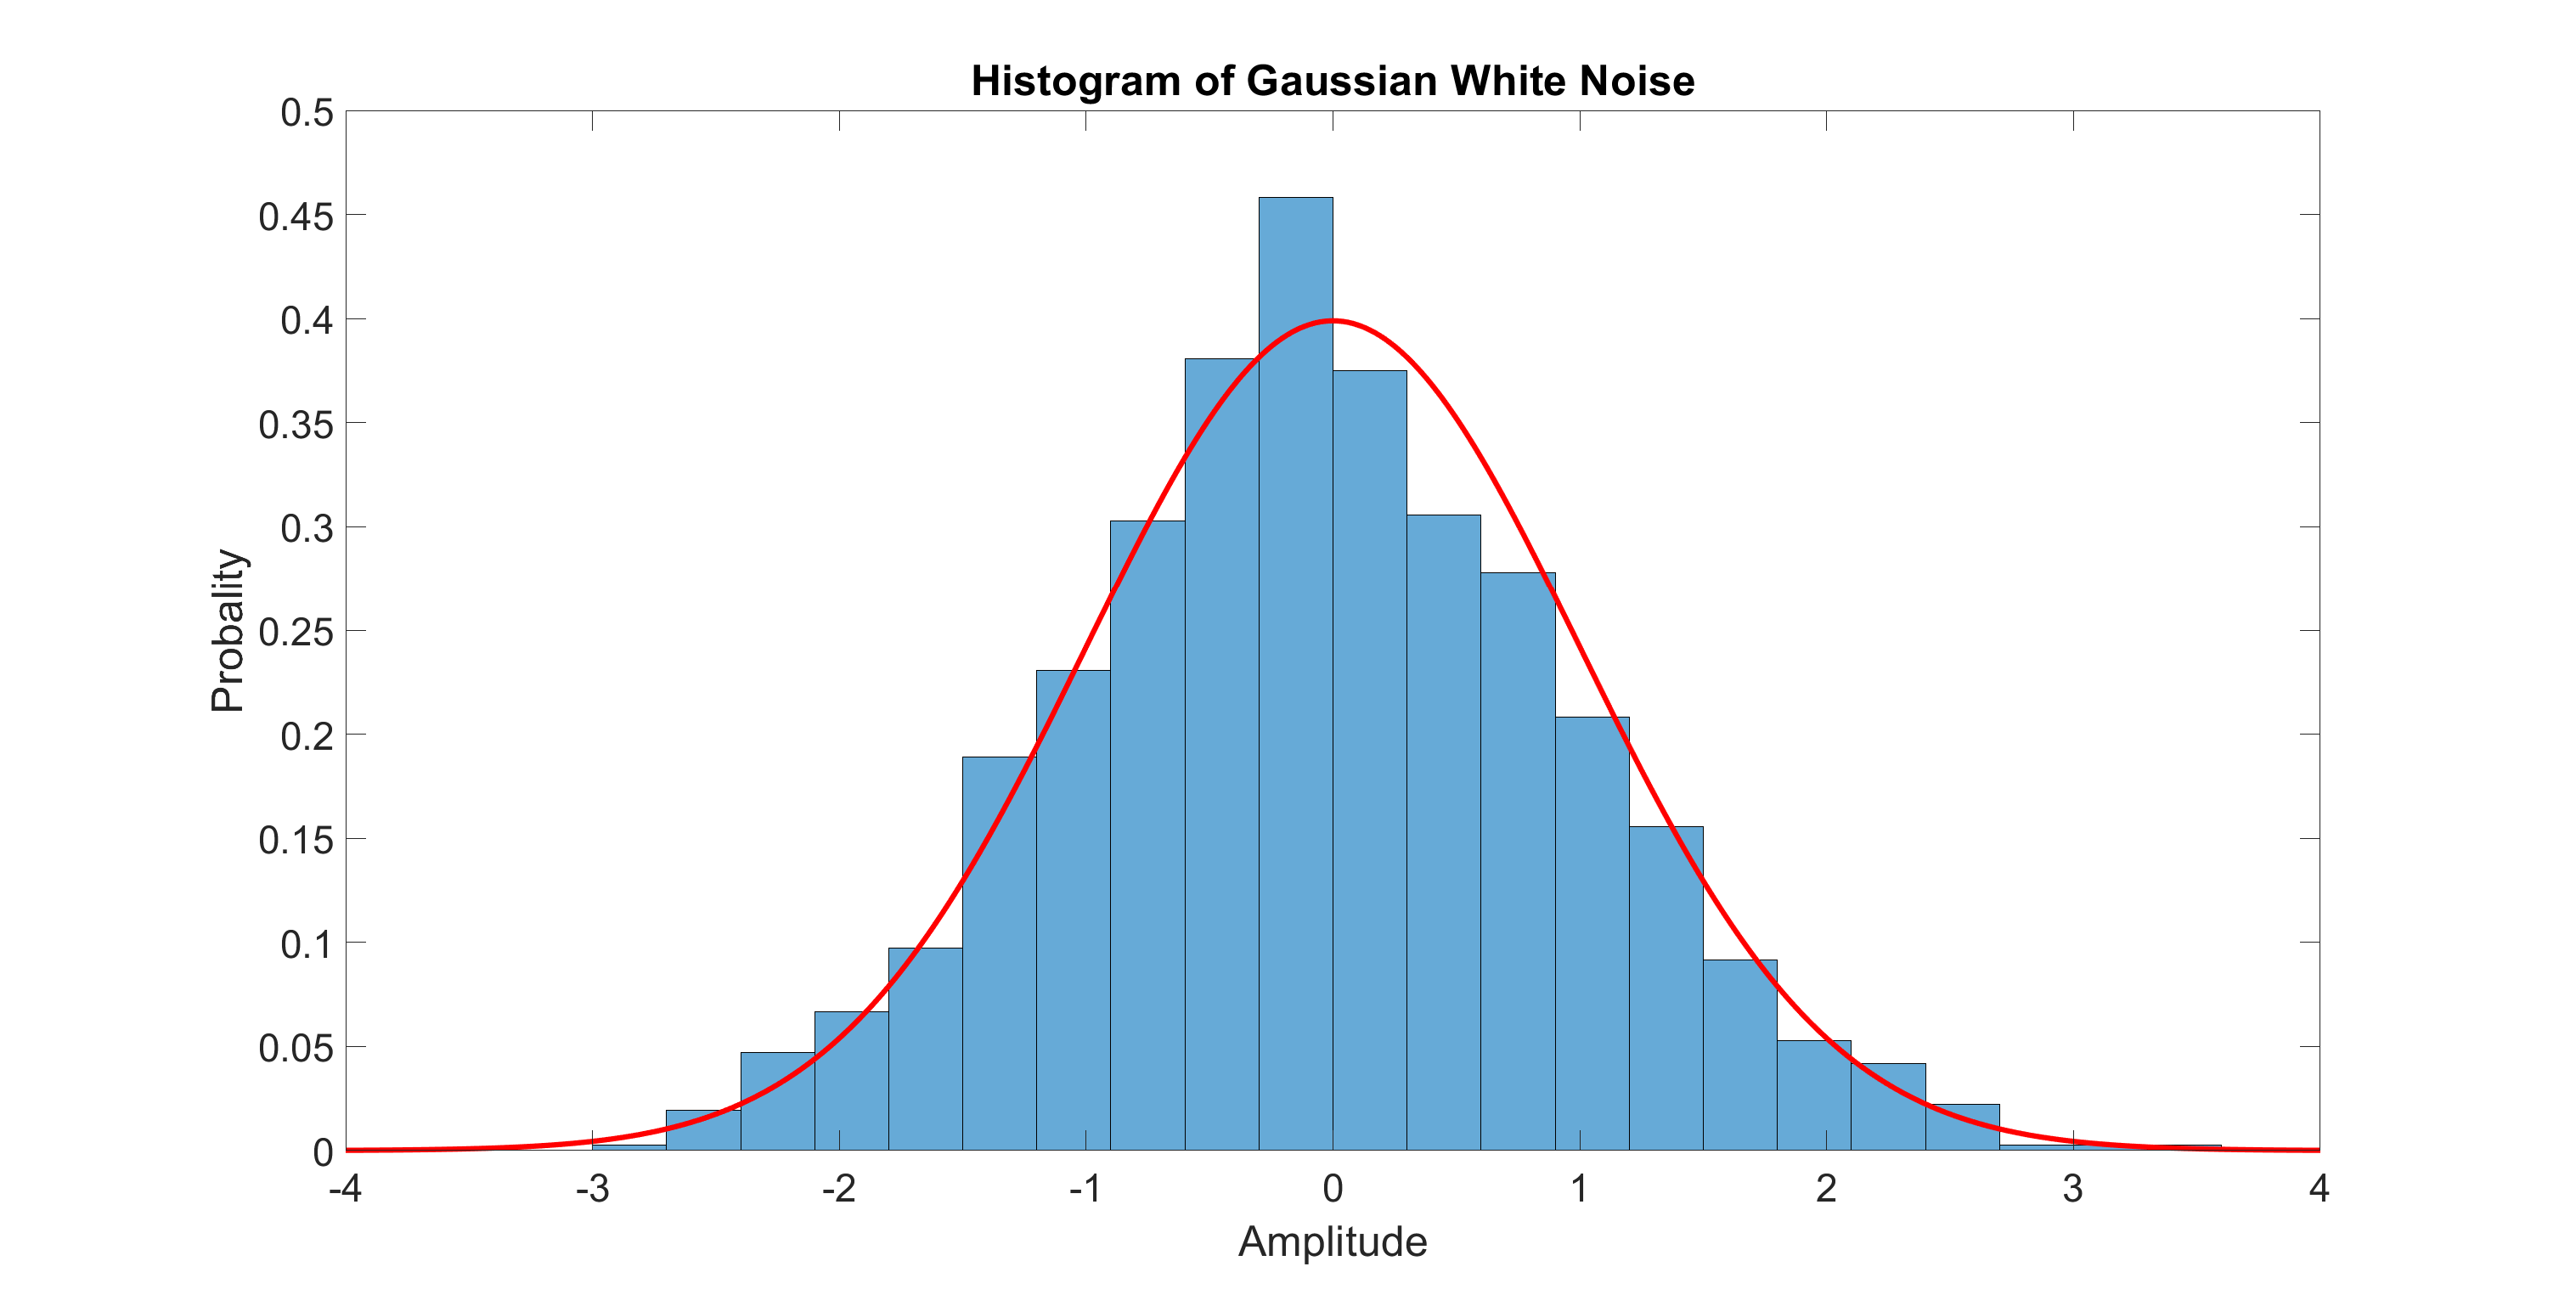
\includegraphics[width=0.7\linewidth]{figure/gwn_histogram}
	\caption{高斯白噪声幅度概率分布}
	\label{fig:gwnhistogram}
\end{figure}
它的功率谱是在频域内均匀分布的,在无限宽频带内满足
\[ G(\omega) = \frac{N_0}{2},\quad -\infty<\omega<+\infty \]
它的自相关函数为为
\[ R(\tau) = \frac{1}{2\pi}\int_{-\infty}^{+\infty}G(\omega)\mathrm{e}^{\mathrm{j}\omega t}\mathrm{d}\omega=\frac{N_0}{2}\delta(\tau) \]

在数字图像中,高斯白噪声线性叠加在图像中。设$f(x, y)$为原图像的表达式,$v(x, y)$为噪声在时空域上的表达式,则包含噪声的图像表达为
\[ g(x, y) = f(x, y) + v(x, y)\]
\subsubsection{傅里叶变换}
傅里叶变换是一种常用的信号分析方法。对于在时空上分布的二数字维图像$f(x, y)$,有傅里叶变换
\[ F(u, v) = \sum_{n = 0}^{N - 1}\sum_{m = 0}^{M - 1}\mathrm{e}^{-\mathrm{j}(\omega_kn+\omega_lm)}f(n, m) \]
对$M\times N$二维灰度图像
\[\begin{pmatrix}
x_{11} & x_{12} & \cdots & x_{1N} \\
x_{21} & x_{22} & \cdots & x_{2N} \\
\vdots & \vdots && \vdots \\
x_{M1} & x_{M2} & \cdots & x_{MN}
\end{pmatrix} \]
进行傅里叶变换,可以得到与图像尺寸相同的$M\times N$复矩阵
\[ \begin{pmatrix}
|A_{11}|\mathrm{e}^{\mathrm{j}\theta_{11}} & |A_{12}|\mathrm{e}^{\mathrm{j}\theta_{12}} & \cdots & |A_{1N}|\mathrm{e}^{\mathrm{j}\theta_{1N}} \\
|A_{21}|\mathrm{e}^{\mathrm{j}\theta_{21}} & |A_{22}|\mathrm{e}^{\mathrm{j}\theta_{22}} & \cdots & |A_{2N}|\mathrm{e}^{\mathrm{j}\theta_{2N}} \\
\vdots & \vdots && \vdots \\
|A_{M1}|\mathrm{e}^{\mathrm{j}\theta_{M1}} & |A_{M2}|\mathrm{e}^{\mathrm{j}\theta_{M2}} & \cdots & |A_{MN}|\mathrm{e}^{\mathrm{j}\theta_{MN}}
\end{pmatrix} \]
其中,靠近中心区域的元素是图片的低频信号幅度和相位,靠近边缘区域的元素是图片的高频信号幅度和相位。
\subsubsection{低通滤波器}
低通滤波器可以滤除高于截止频率的信号分量、保留低于截止频率的信号分量。

对于二维灰度图像,可以设计如图\ref{fig:imagelowpassfilter}低通滤波器
\begin{figure}[H]
	\centering
	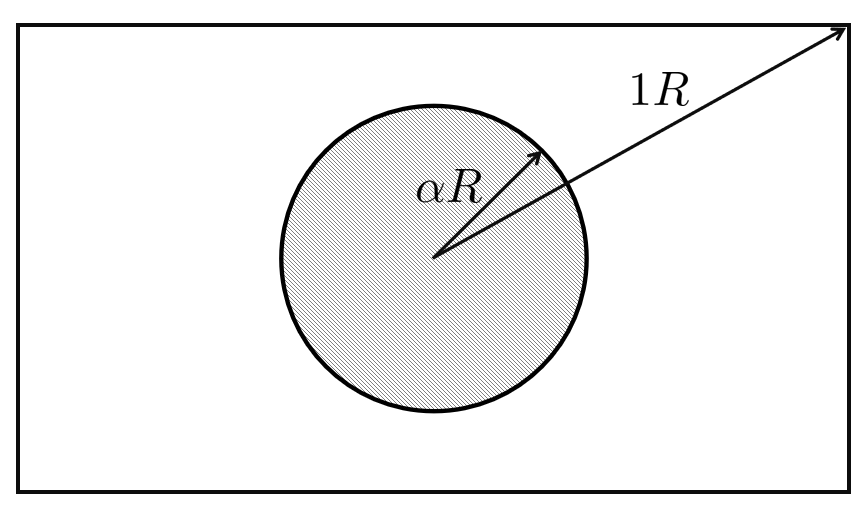
\includegraphics[width=0.7\linewidth]{figure/image_low_pass_filter}
	\caption{二维灰度图的低通滤波器}
	\label{fig:imagelowpassfilter}
\end{figure}
设从图片频域矩阵中心点到一角的距离为$1R$,以图片中心点为圆心,$\alpha R\quad (\alpha \leq1)$为半径作一个圆。保留在圆内信号分量的值,而置圆外元素的值为$0$,最后将图片频域矩阵进行逆傅里叶变换,得到经过低通滤波之后的二维灰度图片。
\subsubsection{均值滤波}
均值滤波是一种线性滤波算法。它是指在图像对目标像素给定一个模板,这个模板包括了它邻域内像素,用这个模板内的像素值代替原来这个像素点处的像素值。如果设均值滤波器的半径为$1$,对于二维灰度图中的某一像素及其邻域为
\[ \begin{pmatrix}
a_{11} & a_{12} & a_{13} \\
a_{21} & A & a_{23} \\
a_{31} & a_{32} & a_{33} \\
\end{pmatrix} \]
则$A$点像素的新的取值为
\[A = \frac{a_{11}+a_{12}+a_{13}+a_{21}+a_{23}+a_{31}+a_{32}+a_{33}}{8}\]
\subsection{实验流程}
\begin{figure}[H]
\begin{subfigure}[b]{0.5\linewidth}
	\centering
\begin{tikzpicture}[node distance=1.5cm]
	\node(start) [startstop] {开始};
	\node(input_img) [io, below of=start, text width=2cm] {读取二维灰度图片};
	\node(add_noise) [process, below of=input_img] {线性叠加高斯噪声};
	\node(fourier_transform) [process, below of=add_noise] {傅里叶变换};
	\node(remove_hf) [process, below of=fourier_transform] {移除高频分量};
	\node(ifft) [process, below of=remove_hf] {逆傅里叶变换};
	\node(output_img) [io, below of=ifft, text width=2cm] {输出滤波后的图片};
	\node(end) [startstop, below of=output_img] {结束};
	
	\draw[arrow] (start) -- (input_img);
	\draw[arrow] (input_img) -- (add_noise);
	\draw[arrow] (add_noise) -- (fourier_transform);
	\draw[arrow] (fourier_transform) -- (remove_hf);
	\draw[arrow] (remove_hf) -- (ifft);
	\draw[arrow] (ifft) -- (output_img);
	\draw[arrow] (output_img) -- (end);
\end{tikzpicture}
\caption{频域低通滤波器流程图}
\label{fig:low_pass_filter}
\end{subfigure}
%\hspace{0.1cm}
\begin{subfigure}[b]{0.5\linewidth}
	\centering
\begin{tikzpicture}[node distance=1.5cm]
	\node(start) [startstop] {开始};
	\node(input_img) [io, below of=start, text width=2cm] {读取二维灰度图片};
	\node(add_noise) [process, below of=input_img] {线性叠加高斯噪声};
	\node(mean_filter) [process, below of=add_noise] {均值滤波};
	\node(output_img) [io, below of=mean_filter, text width=2cm] {输出滤波后的图片};
	\node(end) [startstop, below of=output_img] {结束};
	
	\draw[arrow] (start) -- (input_img);
	\draw[arrow] (input_img) -- (add_noise);
	\draw[arrow] (add_noise) -- (mean_filter);
	\draw[arrow] (mean_filter) -- (output_img);
	\draw[arrow] (output_img) -- (end);
\end{tikzpicture}
\caption{空域均值滤波器流程图}
\label{fig:mean_filter}
\end{subfigure}
\caption{频域滤波器和空域滤波器工作流程图}
\end{figure}
\subsection{实验程序}
\lstinputlisting[caption={向原图添加噪声}]{"../Executable Script/Exp 1/add_noise.m"}
\lstinputlisting[caption={被噪声污染的图片通过滤波器}]{"../Executable Script/Exp 1/process_by_filter.m"}
\lstinputlisting[caption={频域低通滤波器函数}]{"../Function Library/ImageFrequencyDomainLowPassFilter.m"}
\lstinputlisting[caption={空域均值滤波器函数}]{"../Function Library/ImageMeanFilter.m"}
\subsection{实验结果和分析}
用于测试的原图像如图\ref{fig:dji0027gray}所示
\begin{figure}[H]
	\centering
	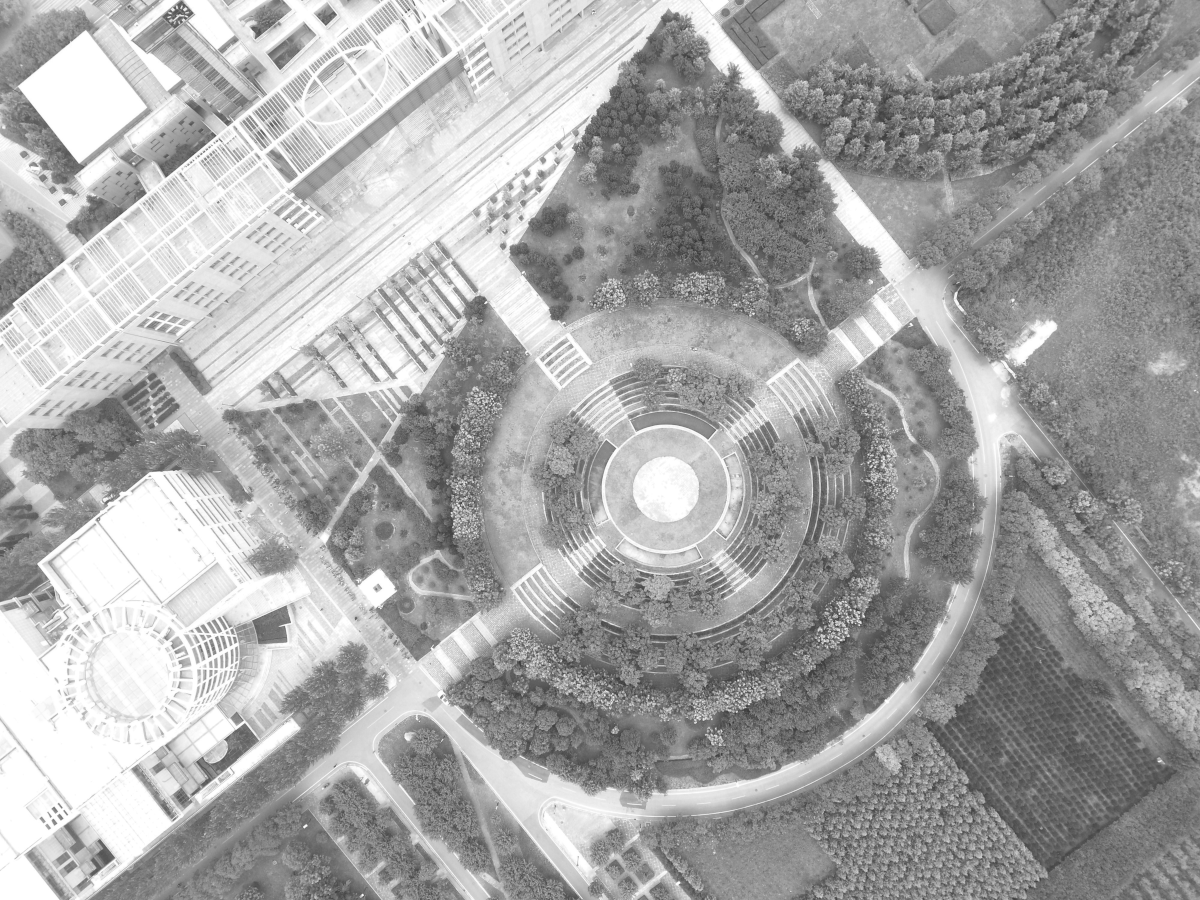
\includegraphics[width=0.7\linewidth]{figure/DJI_0027_Gray}
	\caption{测试原图像}
	\label{fig:dji0027gray}
\end{figure}
在图\ref{fig:dji0027gray}中加入$\sigma^2=0.2^2$的高斯噪声后得到图\ref{fig:dji0027withnoise}
\begin{figure}[H]
	\centering
	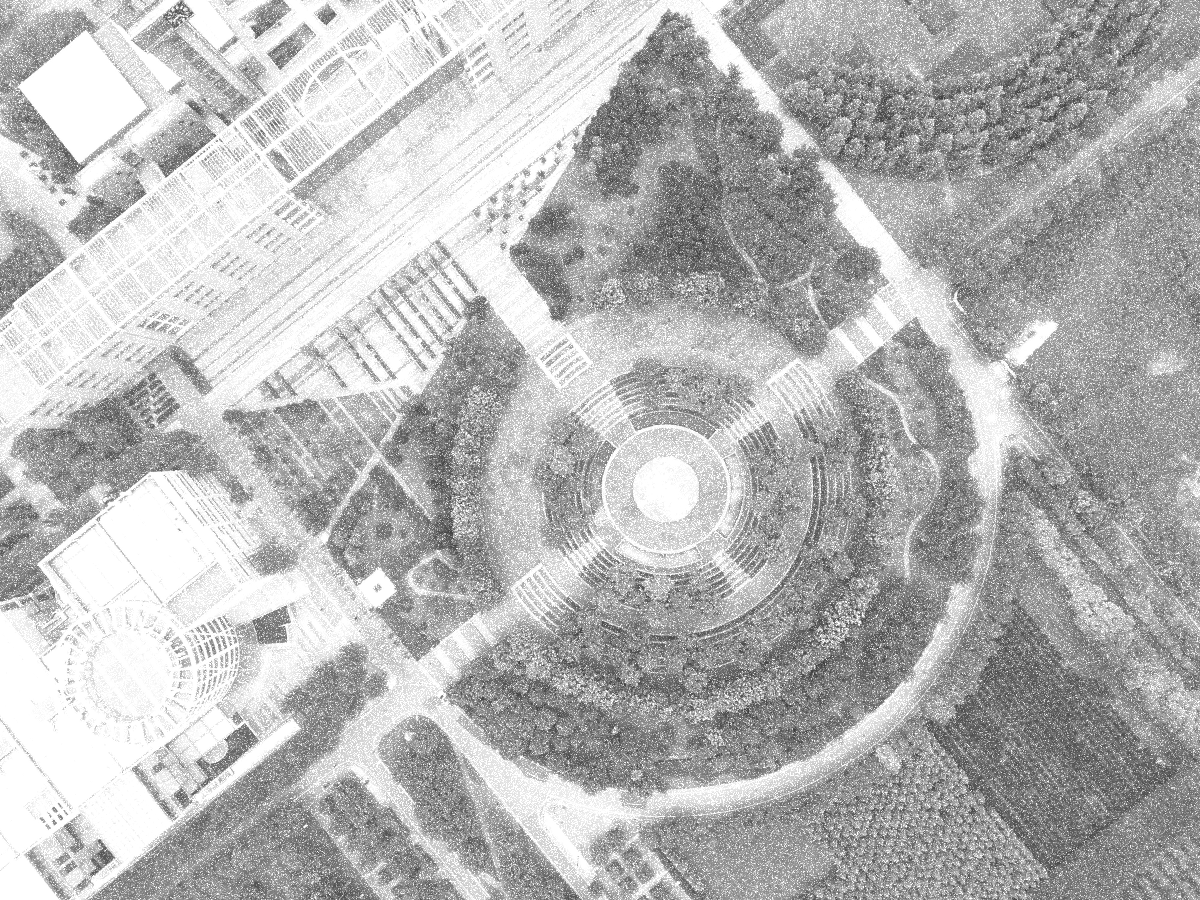
\includegraphics[width=0.7\linewidth]{figure/DJI_0027_With_Noise}
	\caption{加入高斯噪声$\sigma^2=0.2^2$}
	\label{fig:dji0027withnoise}
\end{figure}
使用低通滤波器($r=2$)对噪声图像进行处理,可以得到图\ref{fig:dji0027processedbylp}
\begin{figure}[H]
	\centering
	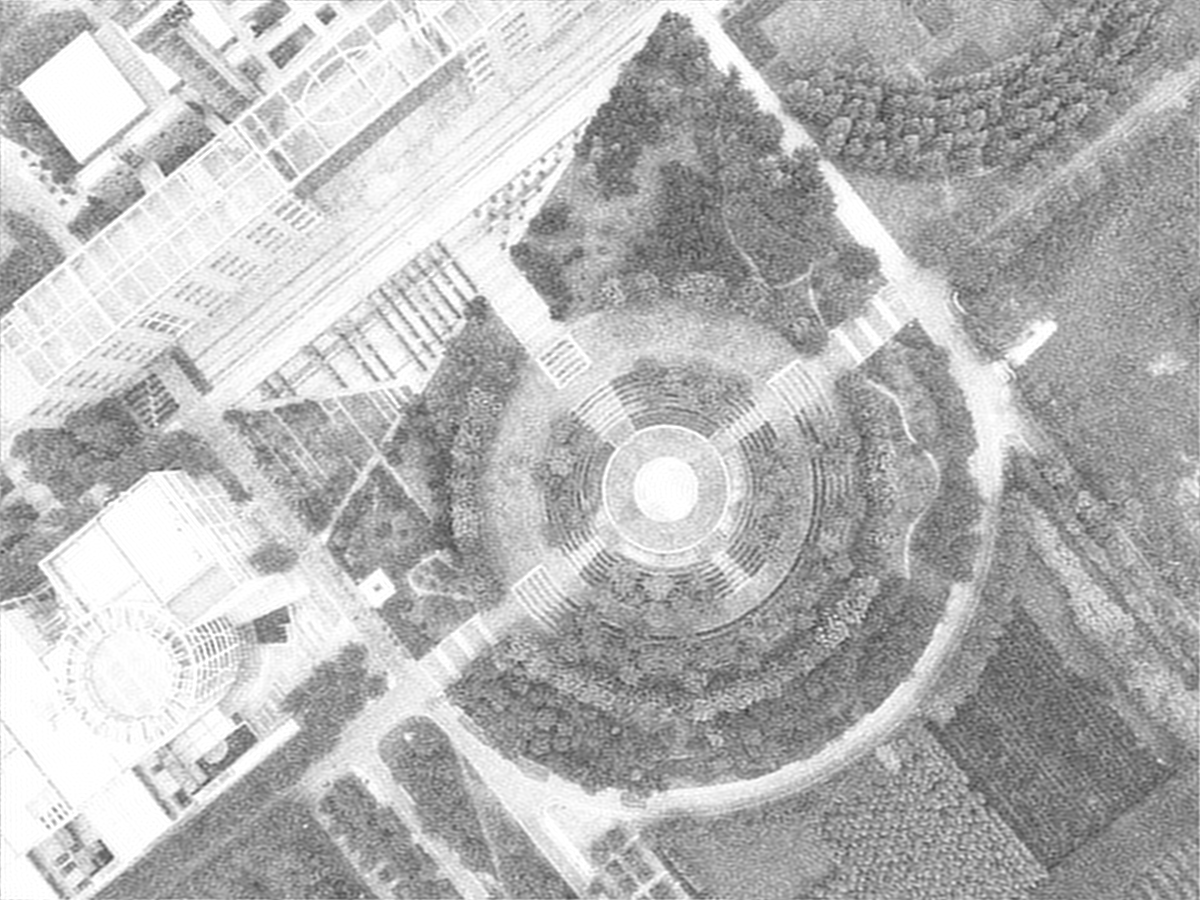
\includegraphics[width=0.7\linewidth]{figure/DJI_0027_Processed_by_LP}
	\caption{低通滤波器($0.5R$)处理之后}
	\label{fig:dji0027processedbylp}
\end{figure}
使用均值滤波器($0.5R$)对噪声图像进行处理,可以得到图\ref{fig:dji0027processedbymf}
\begin{figure}[H]
	\centering
	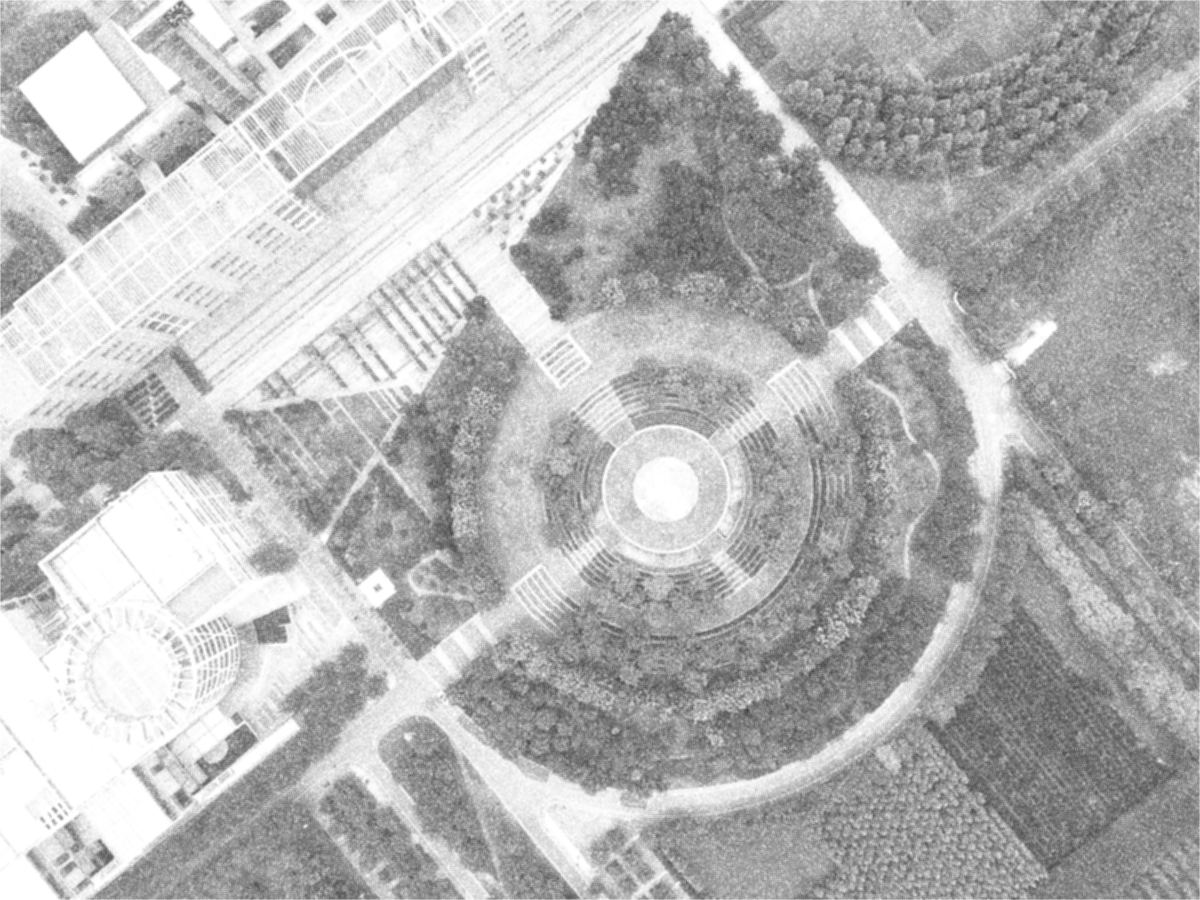
\includegraphics[width=0.7\linewidth]{figure/DJI_0027_Processed_by_MF}
	\caption{均值滤波器($r=2$)处理之后}
	\label{fig:dji0027processedbymf}
\end{figure}
如果加入$\sigma^2=0.5^2$的高斯噪声,可以得到图\ref{fig:dji0027withnoise50}
\begin{figure}[H]
	\centering
	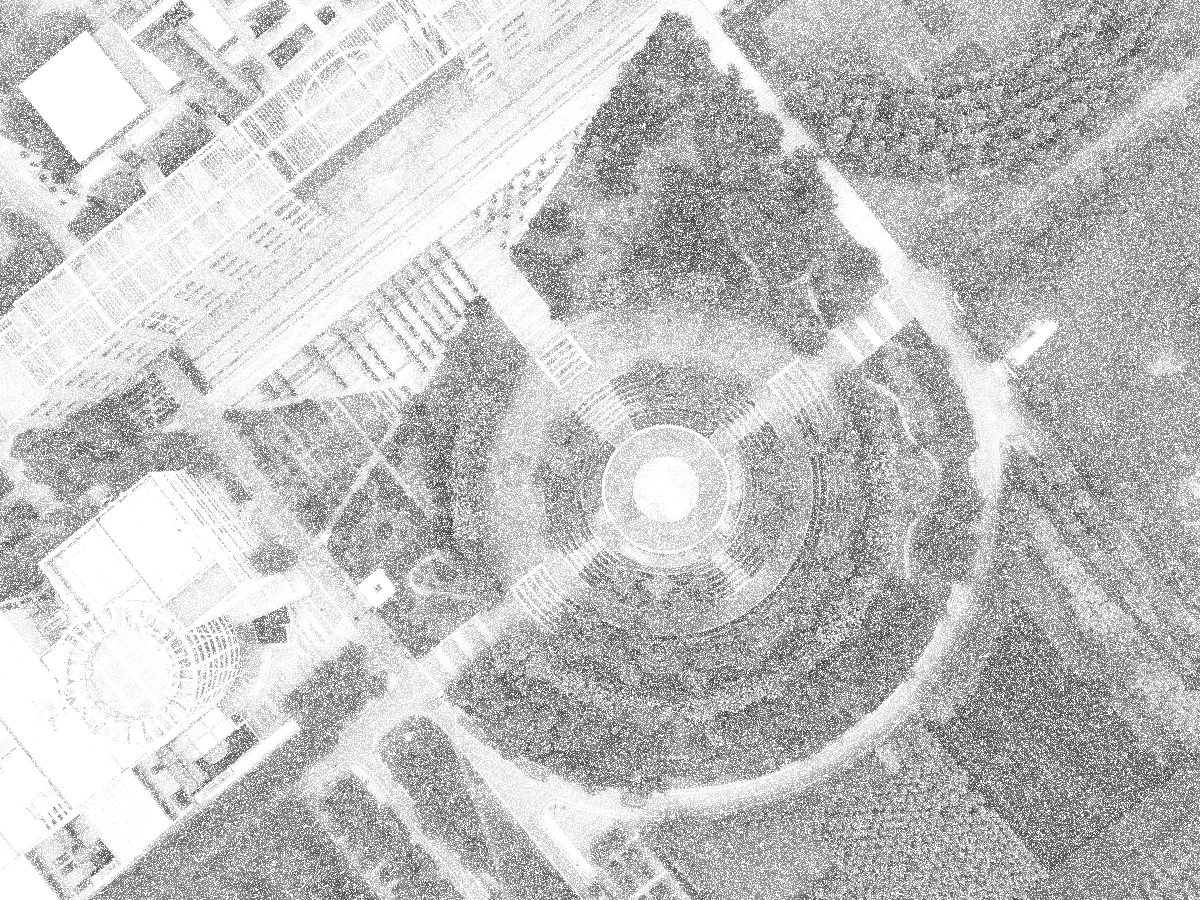
\includegraphics[width=0.7\linewidth]{figure/DJI_0027_With_Noise_50}
	\caption{加入高斯噪声$\sigma^2=0.5^2$}
	\label{fig:dji0027withnoise50}
\end{figure}
使用低通滤波器($r=3$)和高通滤波器($0.3R$)可以得到如图\ref{fig:sigma50}所示的结果
\begin{figure}[H]
	\centering
	\begin{minipage}{0.45\linewidth}
		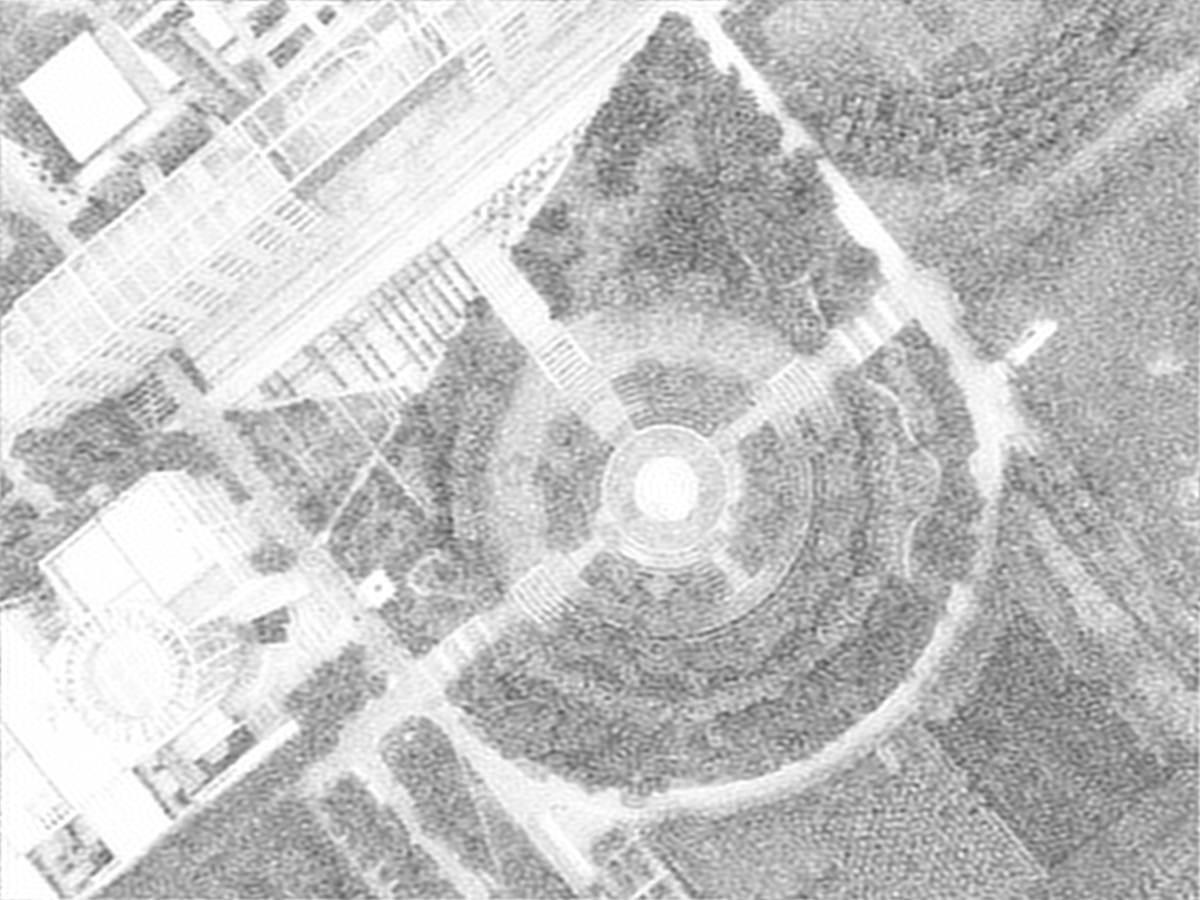
\includegraphics[width=\linewidth]{figure/DJI_0027_Processed_by_LP_50}
		\caption{低通滤波器($0.3R$)处理之后}
	\end{minipage}
	\begin{minipage}{0.45\linewidth}
		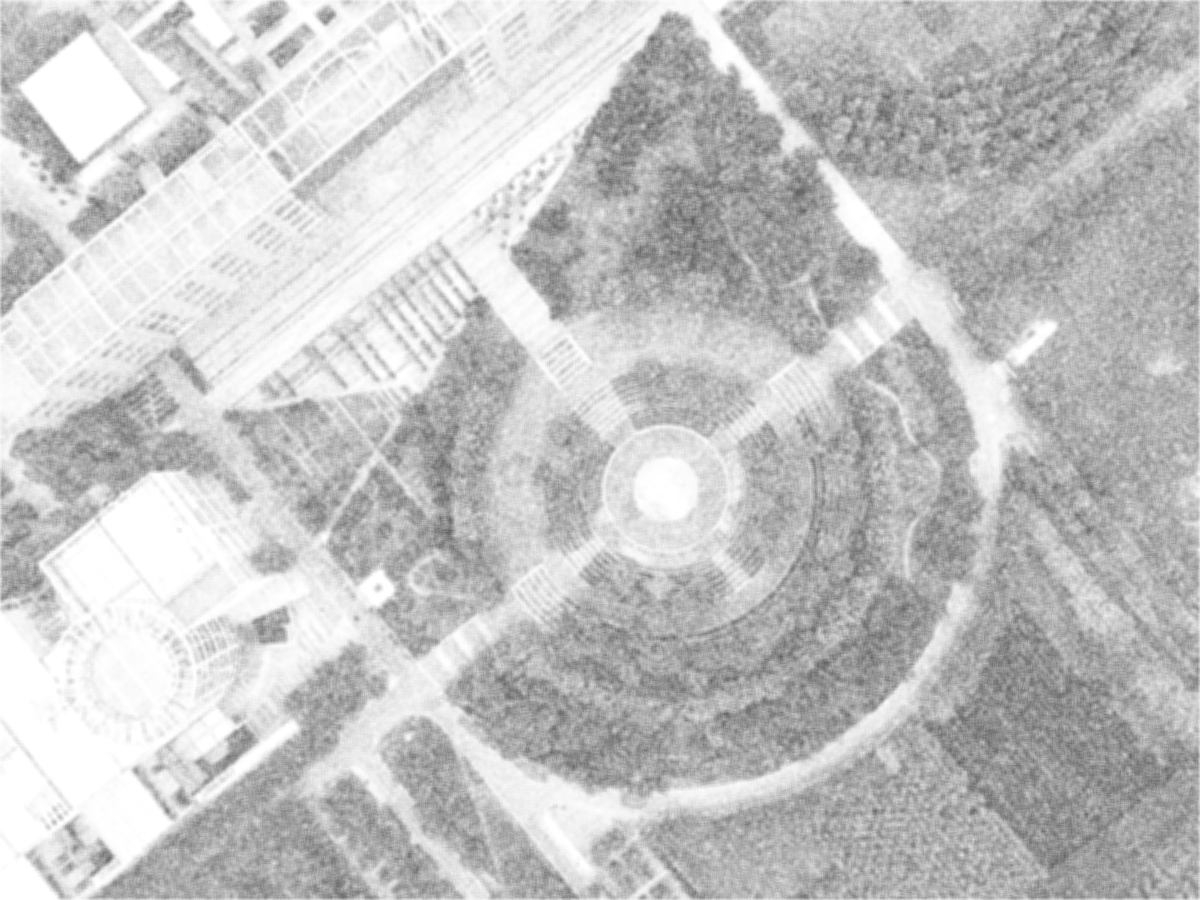
\includegraphics[width=\linewidth]{figure/DJI_0027_Processed_by_MF_50}
		\caption{均值滤波器($r=3$)处理之后}
	\end{minipage}
	\caption{对被$\sigma^2=0.5^2$的高斯噪声污染之后的图像的处理结果}
	\label{fig:sigma50}
\end{figure}
如果加入$\sigma^2=0.7^2$的高斯噪声,可以得到图\ref{fig:dji0027withnoise70}
\begin{figure}[H]
	\centering
	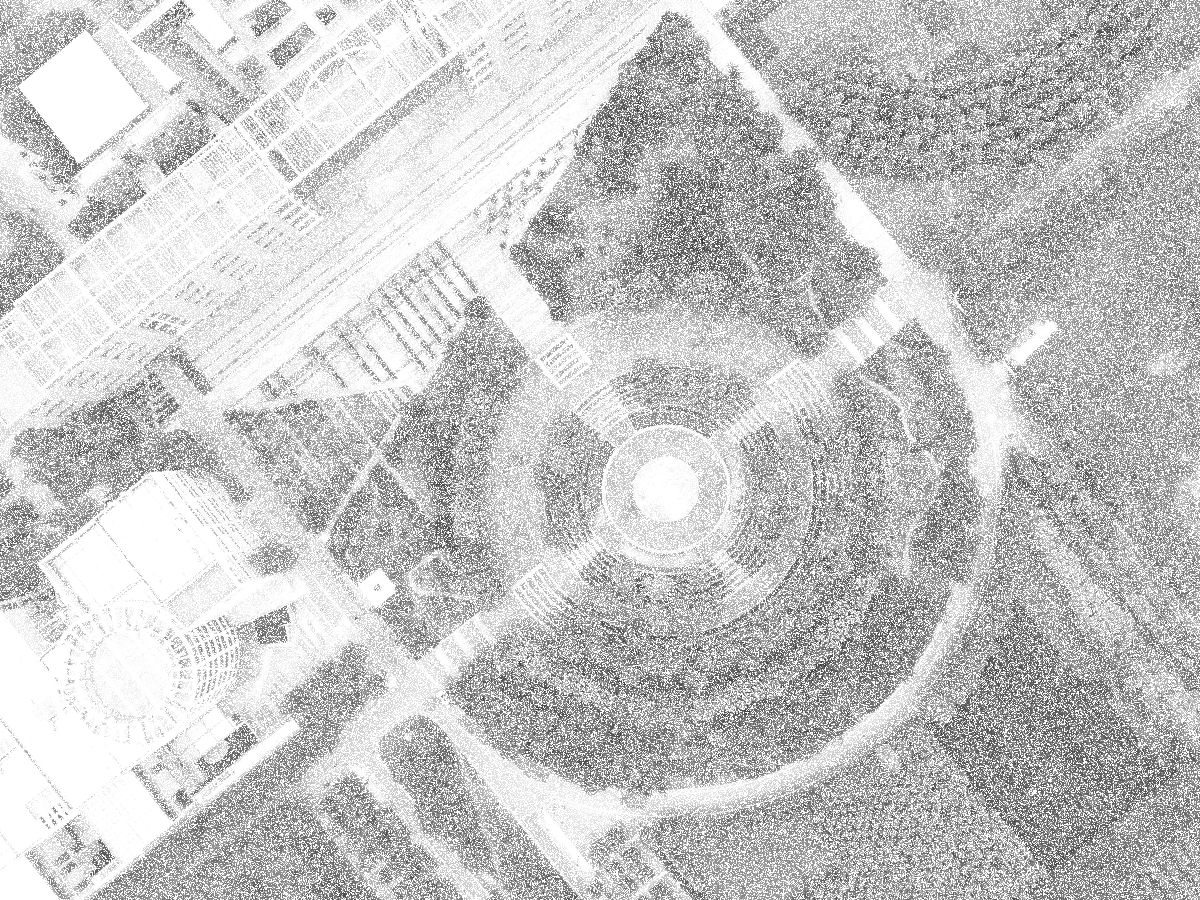
\includegraphics[width=0.7\linewidth]{figure/DJI_0027_With_Noise_70}
	\caption{加入高斯噪声$\sigma^2=0.7^2$}
	\label{fig:dji0027withnoise70}
\end{figure}
使用低通滤波器($r=5$)和高通滤波器($0.2R$)可以得到如图\ref{fig:sigma70}所示的结果
\begin{figure}[H]
	\centering
	\begin{minipage}{0.45\linewidth}
		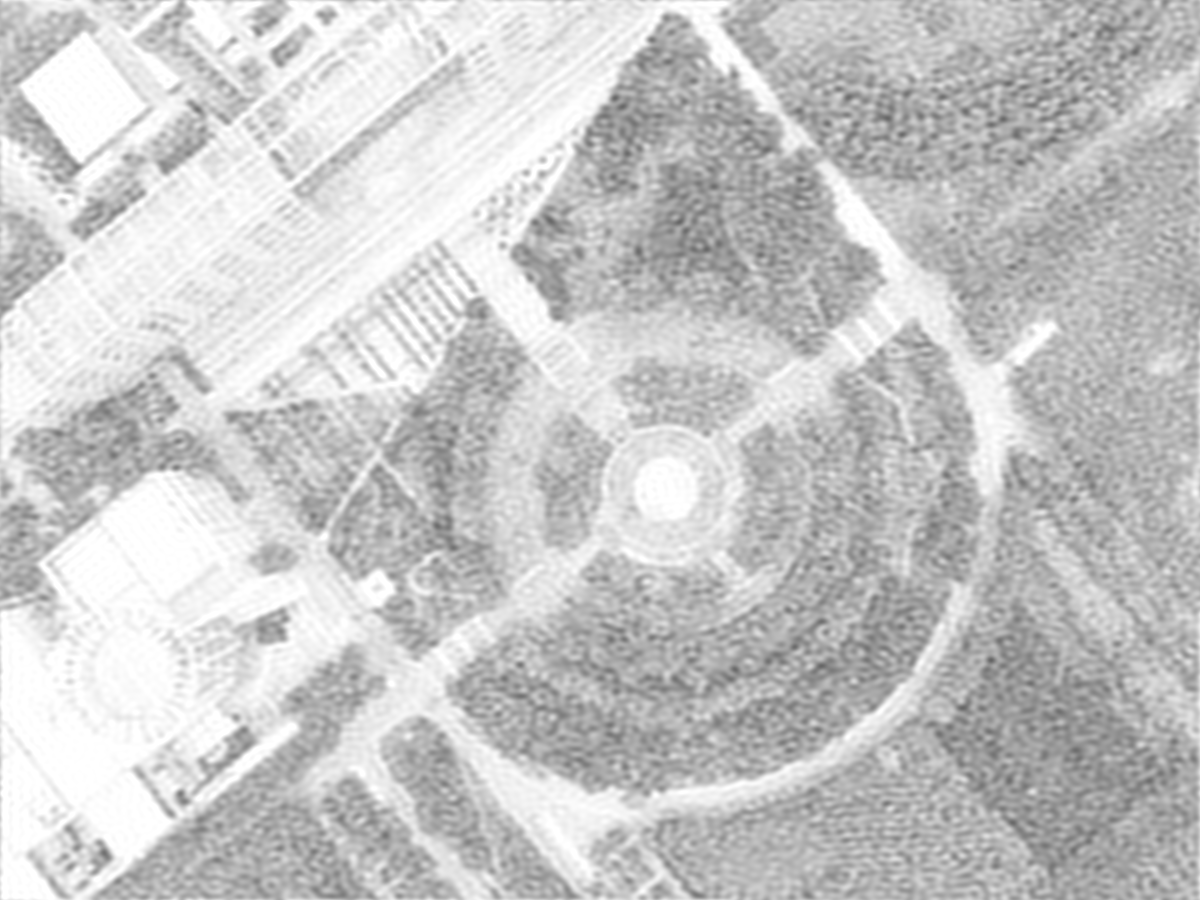
\includegraphics[width=\linewidth]{figure/DJI_0027_Processed_by_LP_70}
		\caption{低通滤波器($0.2R$)处理之后}
	\end{minipage}
	\begin{minipage}{0.45\linewidth}
		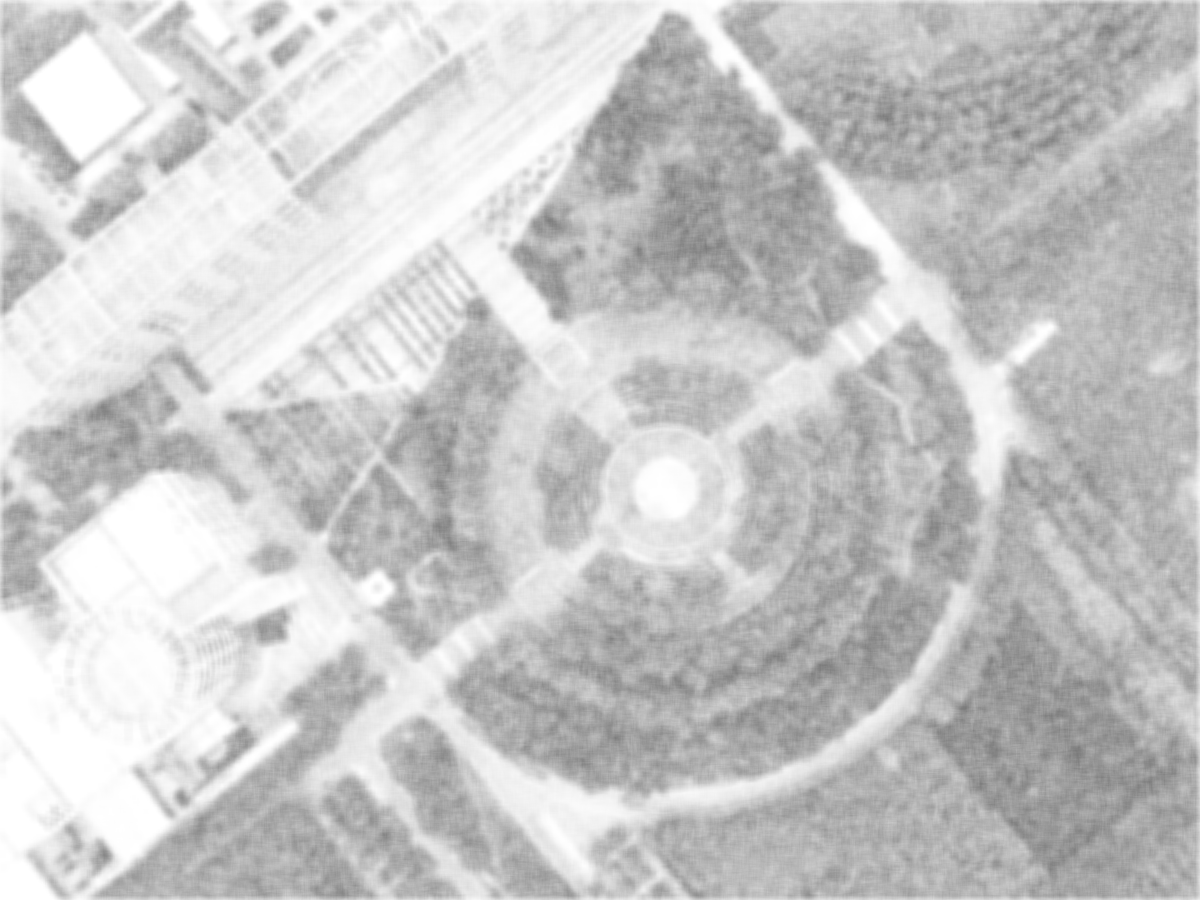
\includegraphics[width=\linewidth]{figure/DJI_0027_Processed_by_MF_70}
		\caption{均值滤波器($r=5$)处理之后}
	\end{minipage}
	\caption{对被$\sigma^2=0.7^2$的高斯噪声污染之后的图像的处理结果}
	\label{fig:sigma70}
\end{figure}
由不同的噪声功率在图像上造成不同的影响并使用不同的滤波器对被污染的图像进行处理可以发现,噪声的功率越大,需要截止频率更低的低通滤波器或半径更大的均值滤波器对图像进行处理,这样才可以得到比较好的降噪结果。在使用低通滤波器的时候,滤波器会消除高于截止频率的信号分量,这可以消除在图片上的高频噪声,但同时也会去除原图片中的高频信号,这就会使得滤波后的图像的边缘、细节丢失。在使用均值滤波器的时候,滤波器会根据每一个点的邻域上像素的取值计算均值作为这一个点的新的像素值,这样可以实现“平滑”图像的效果,即消除在这一区域中突出而尖锐的成分,也就会让原图损失细节特征。